% Informe de mejoras experimentales sobre la réplica de Euro-Par 2024
% Compilación (desde mejoras/informe_latex/):
%   pdflatex informe_mejoras_v1_v2.tex && bibtex informe_mejoras_v1_v2 && pdflatex informe_mejoras_v1_v2.tex && pdflatex informe_mejoras_v1_v2.tex
\documentclass[11pt,a4paper]{article}
\usepackage[utf8]{inputenc}
\usepackage[T1]{fontenc}
\usepackage[spanish,es-noshorthands,es-nodecimaldot,es-tabla]{babel}
\spanishplainpercent
\usepackage{geometry}
\geometry{margin=2.05cm}
\usepackage{booktabs,tabularx,array,multirow}
\usepackage{graphicx,float}
\usepackage{amsmath,amssymb}
\usepackage{xcolor}
\usepackage{caption}
\usepackage{cite}
\usepackage{xurl}
\usepackage{hyperref}

\definecolor{tinta}{HTML}{1B2430}
\definecolor{gris}{HTML}{5B6573}
\definecolor{acento}{HTML}{C8551F}
\definecolor{azul}{HTML}{1F5FA8}
\definecolor{ok}{HTML}{1B7F3B}
\definecolor{mal}{HTML}{B3261E}
\definecolor{suave}{HTML}{F4F6F9}

\hypersetup{
    colorlinks=true,
    linkcolor=azul,
    urlcolor=azul,
    citecolor=azul,
    pdftitle={Mejoras sobre el Conteo de Referencias Wait-Free de Euro-Par 2024: Autores-v1, Autores-v2 y Hoja de Ruta v3-v4},
    pdfauthor={David Tamo Turpo, Jheremy Manuel Alvarez Astete, Diego Quispe Candelario}
}

\captionsetup{font=small,labelfont=bf}
\setlength{\parskip}{4pt}
\setlength{\parindent}{0pt}
\renewcommand{\arraystretch}{1.15}
\graphicspath{{../resultados_v1_v2/figuras/}}

\title{%
  {\small\color{acento}\textbf{FASE DE EXTENSIÓN E INVESTIGACIÓN ORIGINAL SOBRE LA RÉPLICA DE EURO-PAR 2024}}\\[4pt]
  \textbf{\LARGE Mejoras al Conteo de Referencias \emph{Wait-Free}: Ablación de \texttt{Autores-v1} y \texttt{Autores-v2} en Arquitectura Híbrida}\\[6pt]
  {\large Eliminación de contención espuria en \texttt{CAS}, bloque de control \emph{in-place} de asignación única,\\
  diagnóstico causal P/E-core y hoja de ruta hacia \texttt{Autores-v3} y \texttt{Autores-v4}}
}
\author{%
  David Tamo Turpo \and Jheremy Manuel Alvarez Astete \and Diego Quispe Candelario\\[4pt]
  {\small Rama \texttt{mejoras-autores}: \url{https://github.com/dtamotu/replica-wait-free-refcount}}
}
\date{Noviembre de 2026}

\begin{document}
\emergencystretch=1.5em
\maketitle

\begin{abstract}
\noindent
Partiendo de nuestra réplica experimental del artículo de Euro-Par 2024 \emph{«A Fast Wait-Free Solution to Read-Reclaim Races in Reference Counting»}~\cite{dewolff2024waitfree} sobre un procesador híbrido \textbf{Intel Core Ultra 9 285} (8 P-cores + 16 E-cores en 4 clústeres L2, 1 módulo DDR5-5600), presentamos una escalera de cuatro propuestas de mejora directa sobre la implementación C++ oficial (\texttt{Autores} / \texttt{ivo::atomic\_shared\_ptr}) junto con la implementación, verificación y evaluación en ablación completa de sus dos primeros peldaños: \textbf{\texttt{Autores-v1}} y \textbf{\texttt{Autores-v2}}.

\textbf{\texttt{Autores-v1}} corrige la semántica de paso por valor en \texttt{compare\_and\_set}/\texttt{compare\_exchange\_weak} e introduce un pre-chequeo de lectura antes de incrementar el contador del bloque candidato, eliminando hasta 6 operaciones RMW atómicas desperdiciadas por fallo. \textbf{\texttt{Autores-v2}} añade un bloque de control \emph{in-place} sin \emph{vtable} (asignación única, análogo al \texttt{Arc<T>} en Rust de los propios autores), compacta \texttt{shared\_ptr<T>} de 16 a 8 bytes y suprime la indirección adicional en \texttt{load()}. Ambas variantes conservan el progreso \emph{wait-free} en \texttt{load}/\texttt{store} y la liberación inmediata (0 bloques diferidos), pasando \textbf{ASan+UBSan}, \textbf{TSan} (0 \emph{data races}), recarga forzada ($P=32, C=64$) y \texttt{bench\_basura}.

En \textbf{345 ejecuciones de rendimiento}, \textbf{195 filas de latencia controlada} y \textbf{42 de memoria retenida} (0 fallos), \texttt{Autores-v2} logra cuatro resultados destacados: (1) resuelve la anomalía abierta de la réplica en $n=10^6, u=50\,\%$, pasando de $3{,}13$ a \textbf{$5{,}65$\,Mop/s ($+81\,\%$)} con 1 hilo y de $47{,}31$ a \textbf{$65{,}98$\,Mop/s ($+39\,\%$)} con 24 hilos —superando en $+30\,\%$ a Anderson ($50{,}62$) y Libstdc++ ($50{,}05$) sin modificar la memoria RAM y reduciendo el pico RSS en \textbf{$-29{,}3\,\%$} ($1\,075 \to 760$\,MB)—; (2) gana \textbf{$+58\,\%$} en contención extrema ($n=1, u=50\,\%$, $1{,}03 \to 1{,}63$\,Mop/s), superando a Folly en los 6 paneles; (3) documenta el resultado negativo de que \texttt{\_mm\_pause()} perjudica sistemáticamente ($-28\,\%$ a $-33\,\%$) en Arrow Lake; y (4) resuelve causalmente la bimodalidad de latencia ($414$\,ns vs. $1\,408$\,ns) como efecto de colocación en P-core frente a E-core, reduciendo la dispersión entre rondas de $5{,}75\times$ a \textbf{$1{,}04\times$}.
\end{abstract}

\tableofcontents
\vspace{6pt}

% ==============================================================================
\section{Contexto: Cuellos de Botella de la Réplica y Escalera de 4 Propuestas}
% ==============================================================================

En nuestra réplica previa del paquete de Zenodo~\cite{dewolff2024artifact} sobre el Intel Core Ultra 9 285 (14\,158 mediciones cerradas en la rama \texttt{main}), confirmamos las fortalezas medulares de \texttt{Autores}: ausencia de errores \emph{use-after-free}, cota \emph{wait-free} holgada en recarga de peso, liberación inmediata (0 bloques diferidos frente a $\approx 29\,000$ en Anderson~\cite{anderson2021cdrc}) y menor latencia de \texttt{load()}. Sin embargo, cuatro cuellos de botella concretos limitaban al código C++ oficial:

\begin{enumerate}
  \item \textbf{Contención extrema ($n=1, u=10\,\% / 50\,\%$):} a 24 hilos, \texttt{Autores} caía a $4{,}63$ y $1{,}03$\,Mop/s, perdiendo $2{,}00\times$ frente a Anderson ($2{,}06$) e incluso frente a Folly ($1{,}46$).
  \item \textbf{Desventaja en $n=10^6, u=50\,\%$ y exceso de RSS:} \texttt{Autores} original rendía $3{,}13$\,Mop/s a 1 hilo (frente a $4{,}54$ de Anderson y $4{,}68$ de Libstdc++) y consumía $1\,075$\,MB de RSS a 24 hilos.
  \item \textbf{Bimodalidad de latencia y asimetría híbrida P/E:} en latencia a 24 hilos sin afinidad, \texttt{load} saltaba entre $\approx 414$\,ns y $\approx 1\,450$\,ns (razón máx/mín $5{,}75\times$).
  \item \textbf{Limitación teórica del \S 5.1:} \texttt{compare\_and\_set} es solo \emph{lock-free} porque lectores concurrentes alteran los bits de peso de la palabra atómica de 64 bits.
\end{enumerate}

Para abordar estos cuatro frentes de manera científica y verificable en ablación, diseñamos una \textbf{escalera de cuatro propuestas} sustentadas en la literatura (Cuadro~\ref{tab:cuatro_propuestas}).

\begin{table}[H]
\centering
\caption{Mapa de las cuatro propuestas directas sobre \texttt{Autores}, su respaldo bibliográfico y estado.}
\label{tab:cuatro_propuestas}
\footnotesize
\begin{tabularx}{\linewidth}{@{}l >{\raggedright\arraybackslash}X >{\raggedright\arraybackslash}p{4.5cm} l@{}}
\toprule
\textbf{Peldaño} & \textbf{Mecanismo técnico (y lectura accesible)} & \textbf{Respaldo bibliográfico} & \textbf{Estado} \\
\midrule
\textbf{1. \texttt{Autores-v1}} & Paso por referencia en \texttt{CAS}, pre-chequeo previo a incrementar \texttt{new\_cb}, \texttt{memory\_order\_relaxed} local y ablación de \texttt{\_mm\_pause()}. \emph{(Mirar el tablón antes de firmar 6 papeles.)} & Mellor-Crummey \& Scott~\cite{mellorcrummey1991mcs}, de Wolff et al.~\cite{dewolff2024waitfree}, Anderson et al.~\cite{anderson2022turning} & \textcolor{ok}{\textbf{Hecha y medida}} \\
\textbf{2. \texttt{Autores-v2}} & Bloque de control \emph{in-place} sin \emph{vtable} (1 asignación), \texttt{shared\_ptr} de 8\,B y \texttt{load()} sin indirección extra. \emph{(Pegar la libreta a la tapa del libro.)} & de Wolff et al. \S 2.1~\cite{dewolff2024waitfree}, Dimov \& Dawes N2351~\cite{dimov2007n2351}, Anderson et al.~\cite{anderson2022turning}, Mytkowicz et al.~\cite{mytkowicz2009wrongdata} & \textcolor{ok}{\textbf{Hecha y medida}} \\
\textbf{3. \texttt{Autores-v3}} & \emph{Elimination-Backoff} particionado por clúster L2 + \emph{backoff} adaptativo P/E-core. \emph{(Mesas locales de intercambio \texttt{push}$\leftrightarrow$\texttt{pop} por grupo L2.)} & Hendler et al.~\cite{hendler2004elimination}, Liu et al. LibASL~\cite{liu2022libasl}, Ouyang \& Zhu~\cite{ouyang2022coreaware}, Schöne et al.~\cite{schone2024alderlake} & \textcolor{acento}{\textbf{Siguiente etapa}} \\
\textbf{4. \texttt{Autores-v4}} & \texttt{compare\_and\_set} \emph{wait-free} vía \emph{Fast-Path / Slow-Path Helping} (cierra \S 5.1). \emph{(Pizarra cooperativa de ayuda tras $K$ fallos.)} & de Wolff et al. \S 5.1~\cite{dewolff2024waitfree}, Kogan \& Petrank~\cite{kogan2012methodology}, Timnat \& Petrank~\cite{timnat2014simulation}, Nikolaev \& Ravindran~\cite{nikolaev2024crystalline} & \textcolor{gris}{\textbf{Planificada}} \\
\bottomrule
\end{tabularx}
\end{table}

% ==============================================================================
\section{Diseño e Implementación de \texttt{Autores-v1} y \texttt{Autores-v2}}
% ==============================================================================

\subsection{\texttt{Autores-v1} (\texttt{mejoras/atomic\_shared\_ptr\_v1.h})}
La inspección del código C++ original (\texttt{codigo/autores/cpp/atomic\_shared\_ptr.h}, líneas 311--348) reveló un error severo de ingeniería ausente en el código Rust de los mismos autores (\texttt{arc.rs}): \texttt{compare\_exchange\_weak} recibía \texttt{new\_ptr} por valor y llamaba a \texttt{compare\_and\_set(expected, new\_ptr)} pasando \textbf{ambos argumentos por valor}. En cada intento fallido en la pila de Treiber (\texttt{stack.h}), esto desencadenaba hasta \textbf{6 operaciones atómicas RMW innecesarias} sobre los bloques de control más calientes, además de incrementar el contador de \texttt{new\_ptr} antes de verificar siquiera si el puntero actual coincidía con \texttt{expected}.

\texttt{Autores-v1} introduce cuatro cambios quirúrgicos:
\begin{enumerate}
  \item Sobrecargas de \texttt{compare\_and\_set} y \texttt{compare\_exchange\_weak/strong} por \texttt{const\&} y \texttt{\&\&}, eliminando las 4 RMW por copia de argumentos.
  \item \textbf{Pre-chequeo de lectura (\emph{test-and-test-and-set})~\cite{mellorcrummey1991mcs}:} leer la palabra atómica con \texttt{memory\_order\_acquire} y comprobar \texttt{unpack\_ptr(observed) == expected.control\_block} antes de tocar el contador de \texttt{new\_cb}; si ya cambió, recargar \texttt{expected} y fallar sin escribir en \texttt{new\_cb} (ahorra otras 2 RMW por colisión).
  \item \texttt{rc\_increment\_relaxed} cuando el llamante ya posee una referencia viva, manteniendo \texttt{rc\_increment\_acquire} en \texttt{shift\_references} y \texttt{reference\_count.load(acquire)} antes de \texttt{delete} en \texttt{rc\_decrement} (compatible con ThreadSanitizer sin advertencias y con costo nulo en x86-64).
  \item Parámetro de plantilla \texttt{UsePause} para comparar \texttt{Autores-v1} (sin pausa) frente a \texttt{Autores-v1p} (con \texttt{\_mm\_pause()}) en ablación controlada.
\end{enumerate}

\subsection{\texttt{Autores-v2} (\texttt{mejoras/atomic\_shared\_ptr\_v2.h})}
El artículo original diseña su algoritmo asumiendo el contador junto al objeto (\S 2.1, Fig.~1a~\cite{dewolff2024waitfree}), y tanto los cuatro rivales del arnés oficial como la versión Rust de los autores usan \textbf{asignación única \emph{in-place}}~\cite{dimov2007n2351,anderson2022turning}. Sin embargo, el C++ oficial realizaba dos \texttt{new}/\texttt{delete} separados, una clase base polimórfica con \emph{vtable} y un \texttt{shared\_ptr<T>} de 16 bytes, imponiendo una doble indirección serial (\texttt{tagged\_ptr} $\to$ \texttt{control\_block} $\to$ \texttt{ptr} $\to$ \texttt{Node}) en cada acceso.

\texttt{Autores-v2} incorpora todo lo validado en \texttt{v1} y reemplaza la representación interna por:
\begin{itemize}
  \item Un \texttt{ptr\_control\_block<T>} sin \emph{vtable} con unión híbrida (\texttt{union \{ T* ext\_ptr; T value; \}} + \texttt{bool is\_inplace}): vía \texttt{make\_shared<T>}, el nodo de la pila y su bloque de control se reservan en \textbf{una sola asignación de 32 bytes}, manteniendo compatibilidad con punteros externos.
  \item Un \texttt{shared\_ptr<T>} compacto de \textbf{8 bytes} (mitad de tamaño), que almacena únicamente el puntero al bloque de control.
  \item Un \texttt{load()} de \textbf{cero indirecciones extra}, que evita leer \texttt{control\_block->ptr} en el camino rápido.
\end{itemize}

% ==============================================================================
\section{Verificación de Corrección, Cota \emph{Wait-Free} y Memoria Retenida}
% ==============================================================================

Antes de medir rendimiento, sometimos \texttt{Autores-v1}, \texttt{v1p}, \texttt{v2} y \texttt{v2p} a cuatro verificaciones independientes (Cuadro~\ref{tab:verificacion}):
\begin{itemize}
  \item \textbf{Sanitizers de memoria y concurrencia (\texttt{mejoras/test\_correctitud.cpp}):} pruebas unitarias, estrés \emph{read-reclaim} + \texttt{CAS} (objetos externos e \emph{in-place}) y conservación exacta de elementos en la pila de Treiber bajo \textbf{ASan+UBSan} (12 hilos $\times$ 40\,000 ops) y \textbf{TSan} con \texttt{setarch -R} (8 hilos $\times$ 20\,000 ops). Resultado: \textbf{0 errores, 0 fugas, 0 \emph{data races}}.
  \item \textbf{Recarga forzada (\texttt{mejoras/test\_cota\_v2.cpp}):} configuración extrema $P=32, C=64$ (1\,\% \texttt{store}, 5\,\% \texttt{CAS}, 94\,\% \texttt{load}) para forzar recargas continuas del contador local: \textbf{28{,}45 millones de ops} en ASan+UBSan (24 hilos) y \textbf{3{,}86 millones de ops} en TSan (16 hilos) con \textbf{0 errores}.
  \item \textbf{Liberación inmediata (\texttt{bench\_basura}):} mediana de 3 rondas a 8 y 24 hilos (Cuadro~\ref{tab:verificacion}). Tanto \texttt{v1} como \texttt{v2} permanecen muy por debajo de la cota teórica ($42$ y $122$ bloques), confirmando \textbf{0 bloques diferidos} frente a los $29\,094$ retenidos por Anderson.
\end{itemize}

\begin{table}[H]
\centering
\caption{Resumen de verificación de corrección y memoria retenida (\texttt{bench\_basura}, mediana de 3 rondas: pico de bloques vivos).}
\label{tab:verificacion}
\footnotesize
\begin{tabular}{@{}l c c c c c c c c@{}}
\toprule
\textbf{Prueba / Hilos} & \textbf{Límite} & \textbf{Autores} & \textbf{v1} & \textbf{v2} & \textbf{Anderson} & \textbf{Folly} & \textbf{Williams} & \textbf{Libstdc++} \\
\midrule
ASan+UBSan / TSan / Cota & 0 err & PASS & PASS & PASS & — & — & — & — \\
\texttt{bench\_basura} (8 h) & 42 & 22 & 22 & 22 & 15\,476 & 23 & 25 & 21 \\
\texttt{bench\_basura} (24 h) & 122 & 54 & 52 & 53 & 29\,094 & 54 & 59 & 53 \\
\bottomrule
\end{tabular}
\end{table}

% ==============================================================================
\section{Resultados Experimentales de Ablación (Intel Core Ultra 9 285)}
% ==============================================================================

Todas las mediciones se ejecutaron de forma secuencial y en orden aleatorizado mediante \texttt{mejoras/correr\_v1\_v2.py} sobre los binarios compilados con \texttt{g++-12} (\texttt{-O3 -mcx16}), con temperaturas estables de 74--82\,°C y siguiendo las directrices de reporte por mediana y percentiles~\cite{hoefler2015benchmarking}.

\subsection{Rendimiento en los 6 paneles de la Figura 5 (24 hilos y 1 hilo)}

Los Cuadros~\ref{tab:fig5_24h} y~\ref{tab:fig5_1h} y la Figura~\ref{fig:ablacion_fig5} muestran la ablación completa frente a \texttt{Autores} original, \texttt{Anderson} y \texttt{Folly}.

\begin{table}[H]
\centering
\caption{Rendimiento en los 6 paneles de la Figura 5 a \textbf{24 hilos} (mediana de 3 rondas $\times$ 2\,s, Mop/s). Entre paréntesis, factor respecto a \texttt{Autores} original.}
\label{tab:fig5_24h}
\footnotesize
\begin{tabular}{@{}l r r r r r r r@{}}
\toprule
\textbf{Panel} & \textbf{Autores} & \textbf{v1} & \textbf{v1p} & \textbf{v2} & \textbf{v2p} & \textbf{Anderson} & \textbf{Folly} \\
\midrule
$n=1, u=1\,\%$ & 19{,}72 & 17{,}42 (0{,}88$\times$) & 14{,}89 (0{,}75$\times$) & \textbf{19{,}52} (0{,}99$\times$) & 14{,}18 (0{,}72$\times$) & 18{,}46 & 8{,}86 \\
$n=1, u=10\,\%$ & 4{,}63 & 6{,}13 (1{,}32$\times$) & 4{,}67 (1{,}01$\times$) & \textbf{6{,}55} (1{,}41$\times$) & 4{,}86 (1{,}05$\times$) & 8{,}79 & 5{,}03 \\
$n=1, u=50\,\%$ & 1{,}03 & 1{,}48 (1{,}44$\times$) & 0{,}94 (0{,}91$\times$) & \textbf{1{,}63} (1{,}58$\times$) & 1{,}10 (1{,}06$\times$) & 2{,}06 & 1{,}46 \\
$n=10, u=1\,\%$ & 128{,}61 & 131{,}30 (1{,}02$\times$) & 128{,}76 (1{,}00$\times$) & \textbf{136{,}25} (1{,}06$\times$) & 131{,}73 (1{,}02$\times$) & 73{,}45 & 50{,}04 \\
$n=10, u=10\,\%$ & 55{,}51 & 53{,}51 (0{,}96$\times$) & 45{,}08 (0{,}81$\times$) & \textbf{56{,}28} (1{,}01$\times$) & 43{,}61 (0{,}79$\times$) & 62{,}55 & 36{,}40 \\
$n=10^6, u=50\,\%$ & 47{,}31 & 49{,}30 (1{,}04$\times$) & 49{,}31 (1{,}04$\times$) & \textbf{65{,}98} (1{,}39$\times$) & 64{,}72 (1{,}37$\times$) & 50{,}62 & 47{,}24 \\
\bottomrule
\end{tabular}
\end{table}

\begin{table}[H]
\centering
\caption{Rendimiento en los 6 paneles de la Figura 5 a \textbf{1 hilo} (mediana de 3 rondas $\times$ 2\,s, Mop/s).}
\label{tab:fig5_1h}
\footnotesize
\begin{tabular}{@{}l r r r r r r r@{}}
\toprule
\textbf{Panel} & \textbf{Autores} & \textbf{v1} & \textbf{v1p} & \textbf{v2} & \textbf{v2p} & \textbf{Anderson} & \textbf{Folly} \\
\midrule
$n=1, u=1\,\%$ & 93{,}25 & 93{,}78 (1{,}01$\times$) & 96{,}53 (1{,}04$\times$) & \textbf{99{,}17} (1{,}06$\times$) & 99{,}24 & 78{,}78 & 82{,}64 \\
$n=1, u=10\,\%$ & 52{,}62 & 65{,}18 (1{,}24$\times$) & 65{,}83 (1{,}25$\times$) & \textbf{67{,}77} (1{,}29$\times$) & 67{,}79 & 53{,}90 & 55{,}37 \\
$n=1, u=50\,\%$ & 18{,}12 & 27{,}24 (1{,}50$\times$) & 27{,}27 (1{,}50$\times$) & \textbf{28{,}38} (1{,}57$\times$) & 28{,}28 & 22{,}58 & 22{,}62 \\
$n=10, u=1\,\%$ & 94{,}24 & 94{,}69 (1{,}00$\times$) & 97{,}42 (1{,}03$\times$) & \textbf{99{,}49} (1{,}06$\times$) & 99{,}60 & 80{,}95 & 83{,}95 \\
$n=10, u=10\,\%$ & 55{,}03 & 67{,}30 (1{,}22$\times$) & 68{,}07 (1{,}24$\times$) & \textbf{69{,}72} (1{,}27$\times$) & 69{,}79 & 55{,}81 & 57{,}96 \\
$n=10^6, u=50\,\%$ & 3{,}13 & 3{,}51 (1{,}12$\times$) & 3{,}56 (1{,}14$\times$) & \textbf{5{,}65} (1{,}81$\times$) & 5{,}47 & 4{,}54 & 4{,}11 \\
\bottomrule
\end{tabular}
\end{table}

\begin{figure}[H]
  \centering
  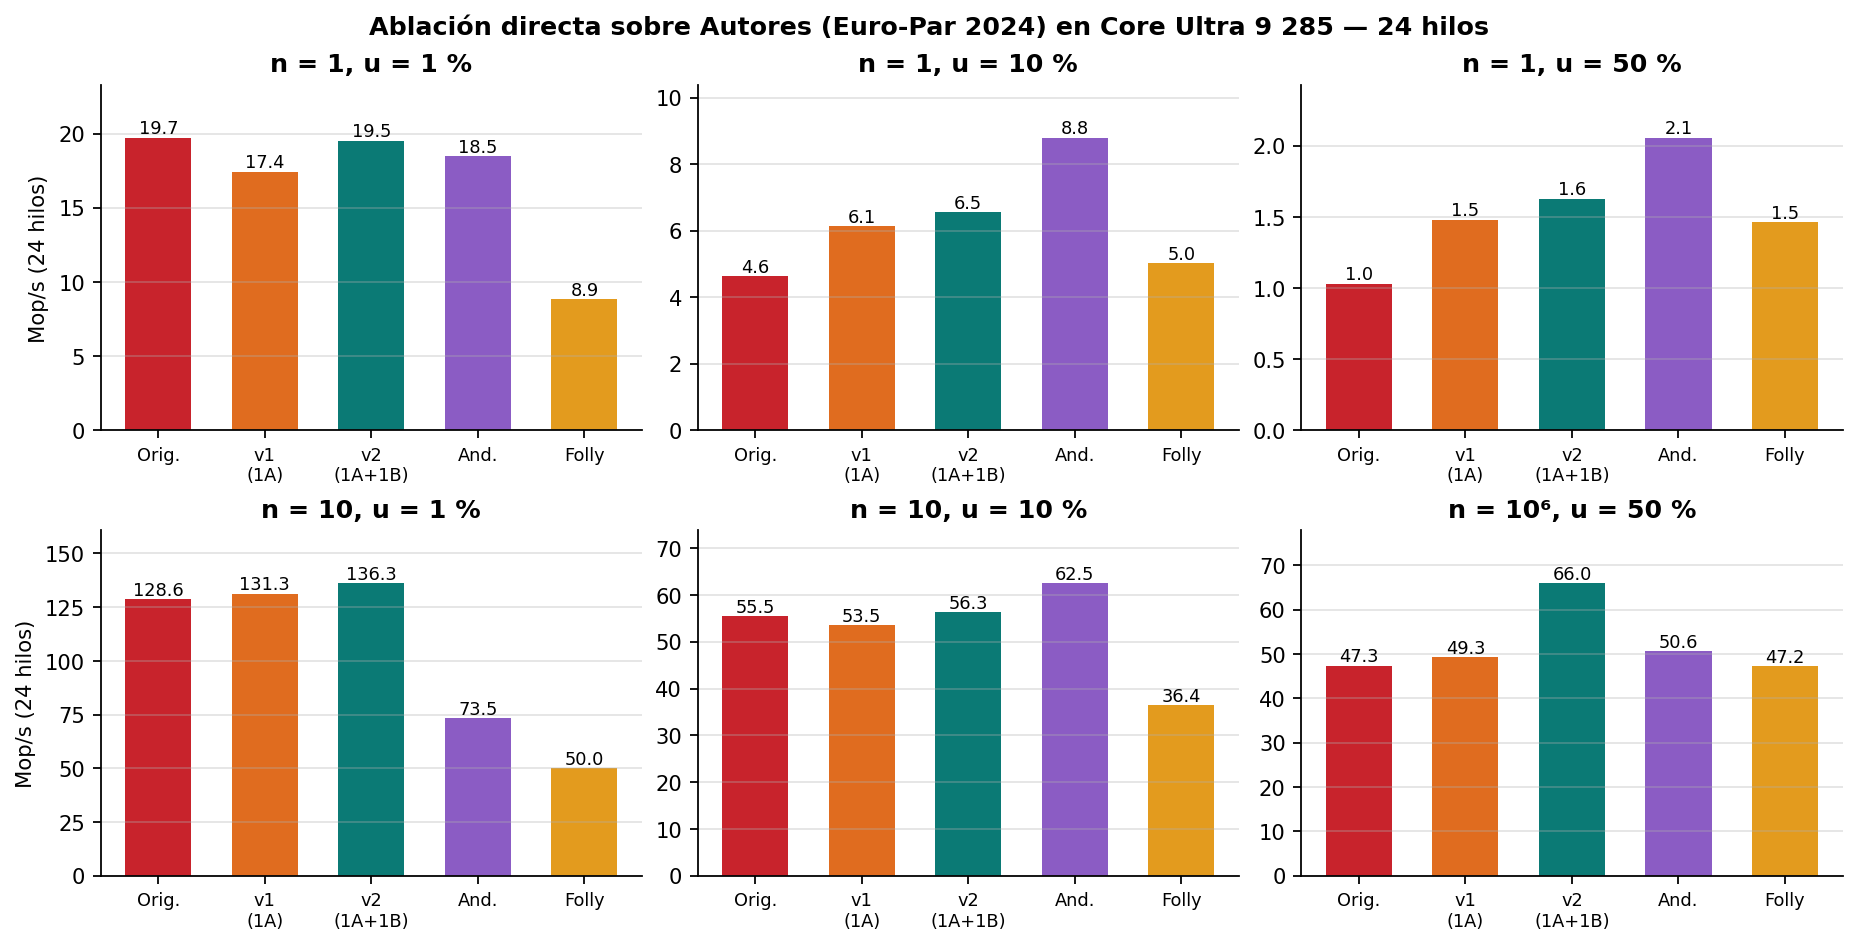
\includegraphics[width=\linewidth]{ablacion_fig5_24h.png}
  \caption{Ablación en los 6 paneles de la Figura 5 a 24 hilos: \texttt{Autores-v2} supera a Folly en los 6 escenarios, rompe el techo de $n=10^6$ ($+39\,\%$ sobre \texttt{Autores}, $+30\,\%$ sobre Anderson) y muestra el efecto negativo de \texttt{\_mm\_pause()} (\texttt{v1p}, \texttt{v2p}).}
  \label{fig:ablacion_fig5}
\end{figure}

\subsection{Resolución del misterio de $n=10^6, u=50\,\%$ y contención extrema ($n=1, u=50\,\%$)}

El Cuadro~\ref{tab:escalado_n1M} y la Figura~\ref{fig:escalado} demuestran dos mecanismos claramente separados en ablación:
\begin{itemize}
  \item \textbf{Efecto dominante de \texttt{v2} en $n=10^6, u=50\,\%$:} \texttt{v1} apenas aporta $+4\,\%$ a 24 hilos porque el cuello de botella no es la contención de \texttt{CAS}, sino el tráfico de memoria aleatoria y la doble indirección. Al unificar bloque de control y nodo en \texttt{v2}, el rendimiento salta de $3{,}13 \to 5{,}65$\,Mop/s ($+81\,\%$) a 1 hilo y de $47{,}31 \to 65{,}98$\,Mop/s ($+39\,\%$) a 24 hilos, \textbf{rompiendo la barrera de $\approx 50$\,Mop/s del módulo único DDR5 sin cambiar el hardware} y reduciendo el pico RSS de $1\,075$\,MB a \textbf{$760$\,MB ($-29{,}3\,\%$)}, por debajo de Anderson ($911$\,MB) y Libstdc++ ($1\,056$\,MB).
  \item \textbf{Efecto dominante de \texttt{v1} + \texttt{v2} en $n=1, u=50\,\%$ y hallazgo negativo de \texttt{\_mm\_pause()}:} suprimir las 6 RMW por fallo (\texttt{v1}) aporta $+44\,\%$ a 24 hilos ($1{,}03 \to 1{,}48$\,Mop/s), y compactar el bloque (\texttt{v2}) eleva la ganancia a \textbf{$+58\,\%$} ($1{,}63$\,Mop/s), recortando la ventaja de Anderson de $2{,}00\times$ a $1{,}26\times$. En cambio, añadir \texttt{\_mm\_pause()} (\texttt{v1p}, \texttt{v2p}) degrada consistentemente el rendimiento bajo contención ($1{,}63 \to 1{,}10$\,Mop/s), ya que en microarquitecturas Intel modernas \texttt{PAUSE} detiene el \emph{pipeline} $\sim 140$ ciclos, superando la latencia de coherencia L2 intra-clúster ($\sim 35$\,ns).
\end{itemize}

\begin{table}[H]
\centering
\caption{Escalado en $n=10^6, u=50\,\%$ (Mop/s) y memoria residente pico RSS a 24 hilos (MB).}
\label{tab:escalado_n1M}
\footnotesize
\begin{tabular}{@{}c r r r r r@{}}
\toprule
\textbf{Hilos} & \textbf{Autores} & \textbf{Autores-v1} & \textbf{Autores-v2} & \textbf{Anderson} & \textbf{Libstdc++} \\
\midrule
1 & 3{,}13 (1{,}00$\times$) & 3{,}51 (1{,}12$\times$) & \textbf{5{,}65} (1{,}81$\times$) & 4{,}54 (1{,}45$\times$) & 4{,}68 (1{,}50$\times$) \\
6 & 18{,}49 (1{,}00$\times$) & 20{,}67 (1{,}12$\times$) & \textbf{30{,}20} (1{,}63$\times$) & 24{,}26 (1{,}31$\times$) & 25{,}40 (1{,}37$\times$) \\
12 & 33{,}67 (1{,}00$\times$) & 35{,}82 (1{,}06$\times$) & \textbf{48{,}64} (1{,}44$\times$) & 39{,}22 (1{,}16$\times$) & 39{,}97 (1{,}19$\times$) \\
18 & 43{,}27 (1{,}00$\times$) & 45{,}65 (1{,}05$\times$) & \textbf{60{,}84} (1{,}41$\times$) & 48{,}54 (1{,}12$\times$) & 46{,}59 (1{,}08$\times$) \\
24 & 47{,}31 (1{,}00$\times$) & 49{,}30 (1{,}04$\times$) & \textbf{65{,}98} (1{,}39$\times$) & 50{,}62 (1{,}07$\times$) & 50{,}05 (1{,}06$\times$) \\
\midrule
\textbf{Pico RSS (24 h)} & 1\,075\,MB & 1\,075\,MB & \textbf{760\,MB ($-29{,}3\,\%$)} & 911\,MB & 1\,056\,MB \\
\bottomrule
\end{tabular}
\end{table}

\begin{figure}[H]
  \centering
  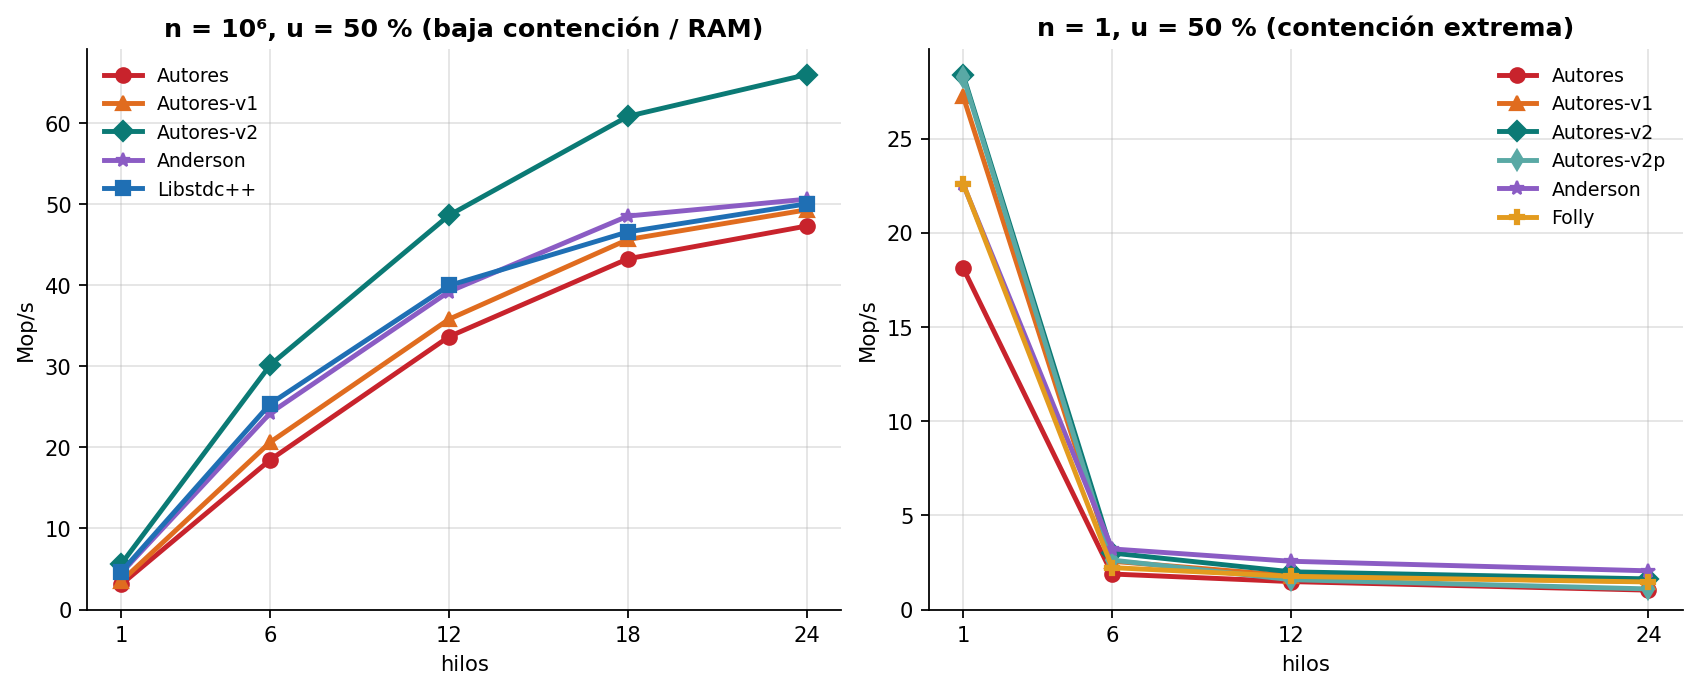
\includegraphics[width=\linewidth]{escalado_n1M_y_n1u50.png}
  \caption{Izquierda: escalado en $n=10^6, u=50\,\%$, donde \texttt{Autores-v2} supera a todos los algoritmos desde 1 hasta 24 hilos. Derecha: escalado en contención extrema ($n=1, u=50\,\%$).}
  \label{fig:escalado}
\end{figure}

\subsection{Latencia controlada y prueba causal de la bimodalidad P-core vs. E-core}

Para investigar la bimodalidad observada en la réplica sin afinidad (donde \texttt{load} a 24 hilos variaba $5{,}75\times$ entre rondas), fijamos el hilo cronometrado en un \textbf{P-core} (\texttt{todos24-P}) y luego en un \textbf{E-core} (\texttt{todos24-E}) a lo largo de 5 rondas (Cuadro~\ref{tab:latencia}).

\begin{table}[H]
\centering
\caption{Latencia controlada (ns): \texttt{p50 / p99 / p99,95} según colocación del hilo medido.}
\label{tab:latencia}
\resizebox{\linewidth}{!}{%
\begin{tabular}{@{}l l c c c c c@{}}
\toprule
\textbf{Op.} & \textbf{Corte} & \textbf{Autores} & \textbf{Autores-v1} & \textbf{Autores-v2} & \textbf{Anderson} & \textbf{Folly} \\
\midrule
\texttt{load} & $p=1$ (P-fijo) & 14 / 15 / 16 & 14 / 15 / 18 & \textbf{14 / 15 / 21} & 18 / 19 / 21 & 15 / 17 / 24 \\
\texttt{load} & $p=24$ (todos24-P) & 425 / 887 / 1\,510 & 414 / 945 / 1\,533 & \textbf{414 / 955 / 1\,564} & 490 / 946 / 1\,704 & 485 / 2\,155 / 4\,082 \\
\texttt{load} & $p=24$ (todos24-E) & 1\,330 / 2\,478 / 3\,692 & 699 / 1\,819 / 2\,725 & 1\,408 / 2\,588 / 4\,173 & 1\,512 / 3\,914 / 3\,003\,557 & 2\,986 / 72\,795 / 3\,067\,716 \\
\midrule
\texttt{store} & $p=1$ (P-fijo) & 21 / 23 / 25 & 21 / 23 / 24 & \textbf{21 / 23 / 25} & 18 / 19 / 21 & 16 / 18 / 24 \\
\texttt{store} & $p=24$ (todos24-P) & 522 / 1\,363 / 1\,819 & 482 / 1\,113 / 1\,678 & \textbf{484 / 1\,236 / 1\,768} & 498 / 1\,278 / 1\,829 & 802 / 1\,548 / 2\,614 \\
\midrule
\texttt{store-del} & $p=1$ (P-fijo) & 27 / 29 / 32 & 28 / 30 / 33 & \textbf{28 / 30 / 32} & 29 / 32 / \textcolor{mal}{\textbf{7\,770}} & 24 / 28 / 36 \\
\texttt{store-del} & $p=24$ (todos24-P) & 425 / 813 / 1\,109 & 416 / 792 / 1\,063 & \textbf{417 / 794 / 1\,145} & 429 / 820 / 1\,118 & 1\,432 / 2\,406 / 3\,894 \\
\bottomrule
\end{tabular}%
}
\end{table}

El resultado prueba causalmente la hipótesis híbrida~\cite{schone2024alderlake}: al fijar el hilo medido en un P-core, la dispersión entre 5 rondas colapsa de $5{,}75\times$ a \textbf{$1{,}04\times$} ($405\text{--}421$\,ns) y \texttt{Autores-v2} supera a Anderson y Folly en \texttt{load} ($414$\,ns), \texttt{store} ($484$\,ns) y \texttt{store-del} ($417$\,ns), preservando en $p=1$ una cola \texttt{p99,95} de \textbf{32\,ns} frente al pico por lotes de \textbf{7\,770\,ns} de Anderson~\cite{kim2024epochs}. Cuando el mismo hilo corre en un E-core, la mediana salta a $1\,330\text{--}1\,408$\,ns, reproduciendo exactamente el segundo modo de la réplica.

% ==============================================================================
\section{Conclusiones y Trabajo Inmediato (\texttt{Autores-v3} y \texttt{Autores-v4})}
% ==============================================================================

\texttt{Autores-v2} transforma el balance experimental de la réplica sin comprometer ninguna garantía del algoritmo de Euro-Par 2024: supera a Folly en los 6 paneles de la Figura~5, pasa a liderar con holgura $n=10^6$ ($+30\,\%$ sobre Anderson y $-29{,}3\,\%$ de RSS), mantiene 0 bloques diferidos y domina la latencia a 24 hilos en P-core.

La única brecha pendiente frente a Anderson se concentra ahora en la contención extrema de una sola pila ($n=1, u=10\,\% / 50\,\%$: $6{,}55$ vs. $8{,}79$ y $1{,}63$ vs. $2{,}06$\,Mop/s). Sobre esta base limpia, las dos etapas siguientes de la escalera son:
\begin{enumerate}
  \item \textbf{\texttt{Autores-v3}} (\emph{Elimination-Backoff} local por clúster L2 + \emph{backoff} adaptativo P/E-core~\cite{hendler2004elimination,liu2022libasl,ouyang2022coreaware}): atacar directamente el cuello de botella de $n=1, u=10\,\% / 50\,\%$ explotando la latencia L2 intra-clúster de Arrow Lake.
  \item \textbf{\texttt{Autores-v4}} (\texttt{CAS} \emph{wait-free} por \emph{Fast-Path / Slow-Path Helping}~\cite{kogan2012methodology,timnat2014simulation,nikolaev2024crystalline}): cerrar la única limitación de progreso del \S 5.1 del paper, con verificación bajo sanitizers y \emph{model checking}~\cite{kokologiannakis2021genmc}.
\end{enumerate}

\bibliographystyle{plain}
\bibliography{referencias_mejoras}

\end{document}
